\documentclass[12pt]{article}
\usepackage{sbc-template}
\usepackage{graphicx}
\usepackage{amsmath}
\usepackage{subfigure}
\usepackage{times,amsmath,epsfig}
\usepackage{graphicx,url}
  \makeatletter
  \newif\if@restonecol
  \makeatother
  \let\algorithm\relax
  \let\endalgorithm\relax
\usepackage[lined,algonl,ruled]{algorithm2e}
\usepackage{multirow}
\usepackage[brazil]{babel}
\usepackage[utf8]{inputenc}
\usepackage[pdftex]{hyperref}

\sloppy

\title{Algoritmos e Estruturas de Dados 3 \\ Trabalho Prático 5 \\
\huge{Cache}}
\date{November 22, 1963}


\author{André Taiar Marinho Oliveira}


\address{Departamento de Ciência da Computação -- Universidade Federal de Minas Gerais (UFMG)
\email{taiar@dcc.ufmg.br}
\\
\\ Novembro de 2010
}

\begin{document}

\maketitle

\begin{resumo}
Este relatório descreve um controlador de hierarquia de memórias e um simulador orientado
a eventos para a geração de requisições de dados que estão gravados nesta memória. Foi simulado 
a requisição de dados que se encontravam em uma camada mais baixa (com alta latência) e utilizado 
um sistema de hierarquia de camadas de memória acima desta com o efeito de uma Cache para o sistema. 
Nessas camadas foram implementadas quatro políticas diferentes de Cache e aplicadas arbitráriamente 
sobre formatos igualmente arbitrários desse sistema. Como resultados pudemos perceber aspectos sobre 
o ganho da eficiência de sistemas que utilizam Cache e como combinações de diferentes tamanhos de caches 
e diferentes políticas de manejo de memória podem funcionar ajudando ou atrapalhando o sistema que a 
utiliza.
\end{resumo}

\section{Introdução}
\textit{"O ideal seria ter uma capacidade de memória infinitamente grande a ponto de qualquer word
específica ... estar imediatamente disponível. ... Somos ... forçados a reconhecer a possibilidade de 
construir uma hierarquia de memórias, cada uma com capacidade maior que a anterior, mas com acessibilidade
menos rápida."} \footnote{A. W. Burks, H. H. Goldstine e J. von Neumann - \textit{Preliminary Discussion of the 
Logical Design of an Electronic Computing Instrument, 1946}}

Hierarquia de memória é, basicamente, uma estrutura organizada em múltiplos níveis de memórias. Tais níveis 
de são diferenciados usualmente por duas dimensões: o tamanho (ou a capacidade de armazenamento daquele
nível) e sua velocidade de acesso (ou sua latência - velocidade com a qual a memória disponibiliza o dado 
assim que ele é requisitado).


\section{Solução Proposta}
\label{solucao_proposta}

O método de Intercalação Balanceada de Vários Caminhos, lê partes arbitrárias do 
aquivo de entrada a ser ordenado (partes essas que cabem em memória principal e 
podem ser manipuladas assim), as ordena e salva em arquivos temporários. Ao final 
do processo, quando todo o arquivo inicial está fragmentado em arquivos temporários
menores e ordenados, começa o processo de intercalação do algoritmo, onde os 
temporários são combinados na solução final obtendo-se o arquivo inicial ordenado.

Intercalar significa combinar dois ou mais blocos ordenados em um único bloco ordenado.
A intercalação, neste caso, é utilizada como uma operação auxiliar na ordenação. O 
processo completo utilizado para a ordenação neste trabalho é o visto no algoritmo 
\ref{alg:ord}.

\begin{algorithm}[h!]
\label{alg:ord}
\begin{footnotesize}

$file \longleftarrow$ aponta para o arquivo de entrada\;
$maxSize \longleftarrow$ máximo de valores a serem lidos\;
$v[maxSize] \longleftarrow$ vetor alocado com o tamanho de $maxSize$\;
$count \longleftarrow 0$\;
$tempId \longleftarrow 0$\;
\tcp{Gera temporários}
\While{houver dados em file}
{
	\While{$count < maxSize$}
	{
		$v[count] \longleftarrow$ READ$(file)$\;
		$count \longleftarrow count + 1$\;
	}
	ORDENA\_EM\_MEMORIA\_INTERNA($v$)\;
	ESCREVE\_TEMP($v, tempId$)\;
	$tempId \longleftarrow tempId + 1$\;
}
\tcp{Intercala}
$temps[tempId] \longleftarrow$ vetor alocado com o tamanho de $tempId$\;
\ForEach{arquivo temporário gerado $F_{i}$}
{
	$temps[i] \longleftarrow$ aponta para conteúdo do arquivo $F_{i}$\;
}
\While{houver dados em algum aquivo temporário $F_{i}$}
{
	$leitura \longleftarrow$ SELECIONA\_MENOR\_VALOR(temps);
	ESCREVE\_SAIDA($leitura$);
}

\caption{Intercalação Balanceada de Vários Caminhos}
\end{footnotesize}
\end{algorithm}

A quantidade máxima de valores a serem lidos a cada iteração na parte da geração
dos temporários foi limitada para efeitos de simulação em $1024 * 1024$ números.
Estes são salvos em um vetor e ordenados em memória interna utilizando o algoritmo
\textit{Quicksort}.

\section{Código}

\subsection{Módulos}
O programa foi separado em quatro módulos:
\begin{itemize}
\item \textbf{Entrada e Saída:} controla a leitura do arquivo de entrada
e a escrita do resultado no arquivo de saída. Também faz a validação dos 
argumentos de entrada pela linha de comando.
\item \textbf{Ordenação:} contém o método de ordenação em memória interna 
(\textit{Quicksort} recursivo).
\item \textbf{Externo:} contém o método de ordenação em memória externa. Utiliza
o módulo Ordenação para ordenar os arquivos parciais.
\item \textbf{Principal:} interagiu com todos os outros módulos retornando erro
quando alguma irregularidade era detectada, controla o fluxo de execução do
programa e mede o tempo de execução total do algoritmo.
\end{itemize}

\subsection{Entrada e saída}
\subsubsection{Linha de comando}
Para não haver problemas com a leitura da linha de comando, foi utilizado um utilitário do
sistema Linux chamado \textbf{getopt} que permite uma leitura mais robusta dos argumentos
passados ao programa. O comando para execução do programa definido para a linha de entrada 
foi:
\begin{verbatim}
#: ./tp4 -i <I> -o <O>
\end{verbatim}
Sendo: 
\begin{itemize}
  \item \textbf{I} - Arquivo de entrada;
  \item \textbf{O} - Arquivo de saída;
\end{itemize}

\subsubsection{Formato da entrada}
Para gerar o arquivo de entrada foi utilizado o script disponibilizado pelos monitores que 
gerava números em ponto flutuante com 15 casas de precisão. Os números devem ser positivos 
(pela própria especificação do problema). Não há restrição quanto à  precisão do número (o 
programa trata isso). Um exemplo de entrada válida seria:
\begin{verbatim}
180.00121515154
0.459887321
0.011115155511150
40.3333
40.3333
0.00001000
\end{verbatim}

\subsubsection{Formato da saída}
A saída do programa é retornada no arquivo de saída especificado pela linha de comando.
É formada por 2 colunas contendo na primeira os valores passados pela entrada, sem repetição
e ordenados e na segunda o valor da CDF calculada para o número da mesma linha na primeira 
coluna. O exemplo da saída gerada pela entrada descrita na sub-sessão anterior seria:
\begin{verbatim}
0.000010    0.00000
0.011115    0.00185
0.459887    0.07665
40.333300    6.72222
180.001215    1.00000
\end{verbatim}

Além disso o programa imprime na saída padrão quais foram os tempos de execução, usuário e sistema
gastos nessa execução:
\begin{verbatim}
tempo de execucao:  0.421001
tempo de usuario: 0.260000
tempo de sistema: 0.120000
\end{verbatim}

\subsubsection{Arquivos temporários e arquivo ordenado}
Para fazer a intercalação, vários arquivos temporários são gerados (dependendo do tamanho do arquivo
de entrada). Tais arquivos são nomeados com o prefixo \textit{"temp\_"} seguidos por um número inteiro
sequencial começando de $1$.

Além disso, ao intercalar os arquivos temporários é criado um arquivo de nome padrão (definido no código
do programa como "ordenado") com o conteúdo do arquivo de entrada ordenado com uma precisão de 5 casas decimais.

Todos os arquivos são gerados no diretório em que o executável se encontra.

\subsection{Compilação}
O compilador utilizado neste trabalho foi o GCC (adotado como padrão para a disciplina) e 
o comando para compilar o programa através do GCC é:
\begin{verbatim}
  #: gcc -o tp4 tp4.c io.c io.h externo.c externo.h ordena.c ordena.h
\end{verbatim}
caso estejam todos os arquivos dentro do mesmo diretório.

Como pedido na especificação, foi feito um arquivo Makefile com o qual é possível compilar
o programa com o comando: 
\begin{verbatim}
  #: make main
\end{verbatim}

E podemos compilar e executar o programa com o comando:
\begin{verbatim}
  #: make run
\end{verbatim}
que fará, além da compilação, com que o programa execute com uma entrada pequena.

\section{Avaliação Experimental}
\label{avaliacao_experimental}

Avaliamos experimentalmente os tempos de execução do programa variando o tamanho da entrada
de arquivos relativamente pequenos até valores que geralmente não cabem nas memórias internas 
dos computadores atuais. Todos os testes foram executados na máquina \textit{fourrier} na rede 
do DCC. Os resultados para os tempos de execução são mostrados na tabela \ref{tempossss} (tamanhos em megabytes 
e tempo em segundos):

\begin{table}[htb]
\centering
\caption{Tabela com os tempos de execução}
\label{tempossss}
\begin{tabular}{|c|c|c|c|}
\hline Tamanhos & Execução & Usuário & Sistema \\ 
\hline 10 & 4,26054320
 & 4,20000000
 & 0,05000000
 \\ 
\hline 50 & 20,93500840
 & 20,78199980
 & 0,14800000
 \\ 
\hline 100 & 41,11264280
 & 40,77800000
 & 0,28600000
 \\ 
\hline 500 & 205,77360860
 & 204,39200120
 & 1,17200000
 \\ 
\hline 1024 & 426,76674180
 & 423,85399780
 & 2,47200000
 \\ 
\hline 2048 & 876,34096680
 & 871,16400160
 & 4,60400000
 \\ 
\hline
\end{tabular} 
\end{table}

Os valores da tabela foram plotados na figura 1.

\begin{figure}[ht!]
\centering
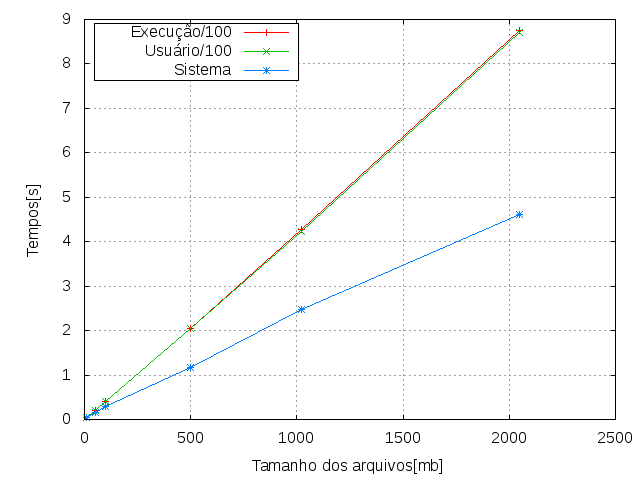
\includegraphics[width=3.5cm,height=2.8cm]{avaliacoes/testes.png}
\label{img:resss}
\caption{Gráfico dos tempos de execução}
\end{figure}

\section{Conclusões}
\label{conclusao}

Neste trabalho foi desenvolvido e analisado um programa que faz a ordenação em memória 
externa de arquivos com números em ponto flutuante. Foi utilizada a memória externa pois o arquivo
geralmente é muito grande para ser ordenado em memória interna, o que torna a resolução do problema
bem mais complexa. Além disso, o arquivo ordenado foi utilizado para calcular a função de probabilidade acumulada do conjunto dos números que foi passado na entrada.

Ao analisar os tempos de execução e visualizar seu comportamento no gráfico, percebemos que variando
o tamanho da entrada o tempo de execução para todas as métricas cresce linearmente. Isso acontece pois
 todos os algoritmos no programa exceto o de ordenação interna têm ordem de complexidade linear (geralmente se resumem a ler arquivos e vetores apenas 1 vez). 
 
Já o algoritmo de ordenação interna que neste caso tem ordem de complexidade $O(n*(log(n)))$ não sofre
 com o aumento da entrada pois todos os vetores que ele ordena têm o mesmo tamanho tornando o seu tempo de execução uma constante no programa, variando linearmente com a entrada.
 
Dessa forma concluímos que a ordenação externa, apesar de lenta se comparada aos algoritmos de ordenação 
em memória interna são extremamente importantes e muito utilizados na prática, em cenários que o tamanho
 dos dados é um fator decisivo. Seu caráter de execução linear mostra que o algoritmo é robusto o
 suficiente para ordenar arquivos bem grandes sem se tornar uma operação inviável (fiz experimentos com arquivos de 20gb que, apesar da demora foram ordenados corretamente).

Por falta de tempo para implementar deixo aqui algumas idéias que fariam análises mais interessantes sobre o assunto e tornaria este trabalho mais proveitoso:
\begin{itemize}
\item Testar o passo de ordenação interna com outros algoritmos (Heapsort por exemplo - por
ser mais estável que o Quicksort). Tal alternativa começou a ser implementada mas teve de ser deixada de lado visto o tempo de entrega do trabalho (vide o módulo \textbf{Ordenação} do programa);
\item Analisar o comportamento do programa para diferentes tamanhos de memória (variar o 
número de itens a serem lidos e ordenados em memória interna);
\item A utilização de paralelismo de dados ou de tarefas poderia ser muito interessante na resolução desse problema uma vez que um grande se encontra no passo da ordenação interna.
\end{itemize}

\end{document}
